\documentclass[journal]{IEEEtran}

\usepackage{cite}
\usepackage{graphicx}
\usepackage{amsmath}
\usepackage{booktabs}
\usepackage{multirow}
\usepackage{array}
\usepackage{url}
\usepackage{xcolor}
\usepackage{enumitem}

\graphicspath{{figures/}}

\begin{document}

\title{An Intraoperative Pulmonary Nodule Localization System Based on Tactile Sensing and Deep Learning: A Frontier Exploratory Study}

\author{Anonymous~Author(s)
\thanks{This Overleaf draft is a working version prepared from the project release package. Author names, affiliations, funding, and ethics statements will be completed in the formal submission version.}}

\markboth{IEEE Transactions on Biomedical Engineering, Draft Version}{Anonymous Author(s): Intraoperative Pulmonary Nodule Localization System}

\maketitle

\begin{abstract}
Minimally invasive thoracoscopic and robot-assisted pulmonary surgery reduces operative trauma, but it also removes the direct tactile feedback that surgeons traditionally rely on to localize hidden nodules. Prior tactile studies on breast and other superficial lesions have shown that internal mechanical heterogeneity can be converted into measurable surface responses under controlled contact. Motivated by this transferable physical principle, we investigated whether flexible tactile sensing could be migrated to intraoperative pulmonary nodule localization, despite the additional challenges posed by lung aeration, collapse, deformation, and mismatch between preoperative CT and intraoperative tissue state. We built a tactile prototype system composed of a flexible array sensor, a front-end acquisition unit, and a workstation, and collected an ex vivo porcine-lung dataset with phantom nodules covering seven sizes, six implantation depths, and three repeated trials. We first used mechanism-guided handcrafted features and an XGBoost baseline to progressively verify whether the tactile data supported nodule detection, size inversion, and coarse depth discrimination, and to identify the dominant physical feature families for each task. We then constructed a raw-input hierarchical neural pipeline that learned directly from spatiotemporal tactile tensors in the order of detection, size prediction, and size-aware coarse depth classification. On the independent test set, the raw-input detector achieved an AUC of 0.8383, exceeding the XGBoost baseline of 0.8199. The raw-input size-only model further surpassed XGBoost on size inversion, achieving top-1/top-2/MAE of 0.7177/0.8195/0.1242 versus 0.6701/0.8023/0.1472. For depth, a shared head again collapsed near majority behavior, whereas a size-aware and route-aware raw-input model improved predicted-route balanced accuracy to 0.5240, surpassing the XGBoost depth baseline of 0.5138; a deployment-oriented unified model further improved this value to 0.5337. Explainability analyses, including latent probes, Integrated Gradients, hard-pair analysis, and phase occlusion, indicated that the network encoded part of the physically meaningful structure related to size and depth, although its temporal strategy still relied heavily on the peak neighborhood. Overall, the study supports a progressive conclusion: tactile spatiotemporal sensing can first support reliable intraoperative pulmonary nodule detection, then size inversion, and under explicit hierarchical organization, cautious coarse depth discrimination. The main contribution lies in establishing a validated, interpretable, and engineering-oriented technical route rather than claiming a finalized clinical system.
\end{abstract}


\begin{IEEEkeywords}
Pulmonary nodule detection, tactile sensing, flexible tactile array, intraoperative navigation, size inversion, coarse depth discrimination, explainable artificial intelligence.
\end{IEEEkeywords}

\section{Introduction}

Low-dose computed tomography has substantially increased the detection rate of small pulmonary nodules and ground-glass lesions. While video-assisted thoracoscopic surgery and robot-assisted surgery have become increasingly important because of reduced trauma and faster recovery, they also remove the direct tactile feedback available in open surgery. As a result, deeply embedded, small, or visually occult nodules become difficult to detect and localize intraoperatively.

Existing clinical support strategies, including CT-guided hook-wire or dye localization, intraoperative ultrasound, and limited digital palpation, all have important limitations. Prior thoracic surgery studies and reviews have emphasized complication risk, marker displacement, operator dependency, and workflow burden as major obstacles to routine use of these approaches \cite{khereba2018preoperative,tang2022intraoperative,wang2025anchored}. Thus, what is missing is not simply another imaging aid, but a sensing pathway that can restore tactile information under minimally invasive conditions and convert it into quantitative guidance.

Flexible tactile arrays offer a promising route toward this goal. By continuously recording the surface stress distribution of the lung during dynamic pressing, such arrays produce spatiotemporal tactile tensors rather than single-point measurements. When a stiff inclusion is embedded inside soft tissue, the mechanical mismatch perturbs peak amplitude, spread extent, shape contrast, deformation position, and temporal response. In principle, these signals may contain three levels of information: whether a nodule is present, how large it is, and how deeply it is buried.

However, the inversion from surface tactile maps to internal nodule parameters is ill-posed. A small shallow nodule may produce a tactile hotspot similar to that of a large deep nodule at a specific pressing frame. Therefore, we do not treat detection, size, and depth as equally difficult parallel outputs. Instead, we formulate the problem hierarchically: \emph{detect the nodule first, estimate its size next, and only then discriminate coarse depth under the size condition}.

Related work in minimally invasive tactile tumor localization, force-reflection integration, and emerging tactile sensing technologies has shown that mechanical differences can be exploited for hidden mass localization \cite{perri2009robot,trejos2013integration,ly2025acoustic,huang2020tactile,bewley2022tactile}. Yet, most prior studies have focused on single localization tasks, simplified phantoms, or hardware feasibility. Fewer studies have organized pulmonary tactile sensing into a full evidence chain spanning reliable detection, size inversion, coarse depth discrimination, raw-input learning, and interpretability verification in the same study.

Motivated by this gap, we follow a five-step logic: mechanism analysis, structured baseline modeling, raw-input neural learning, interpretability validation, and deployment enhancement. First, we analyze whether the tactile data truly contain structured signals for detection, size, and depth. Second, we use XGBoost as a structured baseline to test whether these signals are learnable and to identify the most influential physical feature families. Third, we construct a raw-input hierarchical neural pipeline that learns directly from spatiotemporal tactile tensors without explicitly feeding handcrafted physical features into the scientific main model. Fourth, we examine whether the neural representation automatically encodes physically meaningful structure using latent probes, hard-pair analysis, and phase occlusion. Finally, for deployment purposes, we augment the system with a structured feature branch to improve route-aware robustness in real predicted-size conditions.

The key point is that XGBoost and neural networks serve different purposes in this work. XGBoost is used as a structured mechanistic baseline and interpretability anchor rather than a final deployment model. The raw-input neural models are used to test whether the original tensors themselves are sufficient for learning. The unified hybrid model is then used as a deployment enhancement model rather than the sole proof of raw-input automatic learning.

The main questions we aim to answer are therefore:
\begin{enumerate}[leftmargin=18pt]
\item Can flexible tactile spatiotemporal data support reliable intraoperative pulmonary nodule detection?
\item Beyond detection, can the same data support size inversion and coarse depth discrimination?
\item Without explicitly inputting handcrafted physical features, can a raw-input neural model learn these signals directly from tactile tensors?
\item If so, does the neural representation encode physically meaningful structure consistent with the structured baseline?
\end{enumerate}

The main contributions of this exploratory study are summarized as follows:
\begin{enumerate}[leftmargin=18pt]
\item We establish a structured spatiotemporal tactile dataset and label protocol for intraoperative pulmonary nodule detection, size inversion, and coarse depth discrimination.
\item We show through mechanism analysis and XGBoost that the tactile data contain stable detection information, strong size information, and learnable but weaker depth information.
\item We demonstrate that a raw-input hierarchical neural network can support reliable detection, strong size learning, and size-aware coarse depth discrimination without explicitly feeding structured physical features into the scientific main model.
\item We build an interpretability chain from mechanism-guided features to XGBoost explanations and then to neural latent representations.
\item We further construct a deployment-oriented unified hierarchical inverter that improves predicted-route depth robustness for real-time system integration.
\end{enumerate}

\begin{figure*}[t]
    \centering
    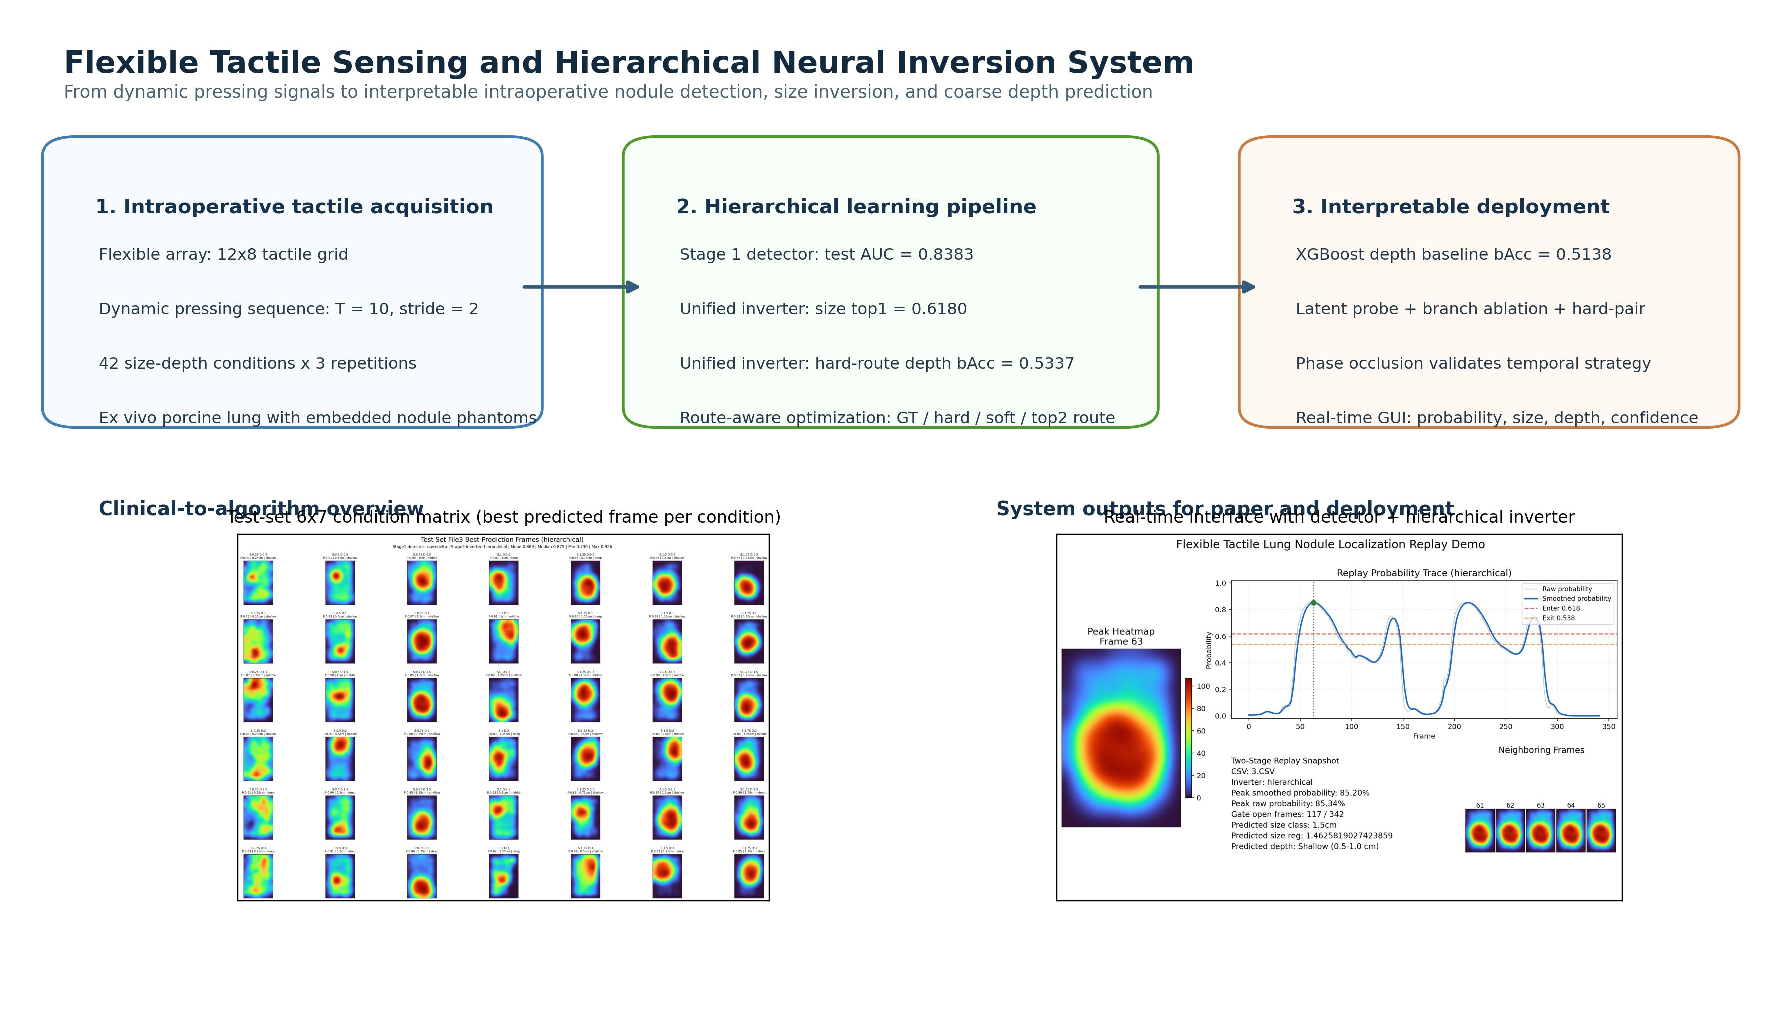
\includegraphics[width=\textwidth]{Fig1_system_overview.pdf}
    \caption{Overall system concept for intraoperative tactile pulmonary nodule localization. The figure summarizes the clinical problem, tactile sensing route, hierarchical model organization, and system-level decision support path.}
    \label{fig:system_overview}
\end{figure*}

\section{Materials and Methods}

\subsection{Experimental Platform and Data Protocol}
Dynamic pressing experiments were performed on ex vivo porcine lungs using a flexible tactile sensing system. Each frame contained 96 sensing channels and was reshaped into a $12 \times 8$ tactile stress matrix. The experimental matrix included seven nodule sizes (0.25 to 1.75 cm), six implantation depths (0.5 to 3.0 cm), and three repeated trials, resulting in 42 physical conditions and 126 full tactile sequences in total.

We used a sliding window of 10 frames with a stride of 2 as the basic learning unit. Detection labels were defined by whether the center frame of a window lay inside the manually annotated positive interval. Size and depth labels were inherited from the corresponding physical condition. Detection used \texttt{1.CSV + 2.CSV} for development and \texttt{3.CSV} for independent testing, whereas size and depth tasks followed a stricter repeat split: \texttt{1.CSV} for training, \texttt{2.CSV} for validation, and \texttt{3.CSV} for testing, all restricted to true positive windows.

\begin{table}[t]
\caption{Dataset protocol and task definition.}
\label{tab:protocol}
\centering
\begin{tabular}{p{0.42\columnwidth}p{0.45\columnwidth}}
\toprule
Item & Value \\
\midrule
Frame size & $12 \times 8$ \\
Channels per frame & \textbf{96} \\
Nodule size levels & \textbf{7 (0.25--1.75 cm)} \\
Depth levels & \textbf{6 (0.5--3.0 cm)} \\
Repeated trials & \textbf{3} \\
Total physical conditions & \textbf{42} \\
Total recorded sequences & \textbf{126} \\
Window length & \textbf{10 frames} \\
Window stride & \textbf{2} \\
Detection split & \textbf{1.CSV + 2.CSV dev, 3.CSV test} \\
Detection windows (train / val / test) & \textbf{4648 / 1107 / 3747} \\
Detection positives (train / val / test) & \textbf{1328 / 223 / 961} \\
Size/Depth split & \textbf{1.CSV train, 2.CSV val, 3.CSV test} \\
Size/Depth training samples & \textbf{true positive windows only} \\
\bottomrule
\end{tabular}
\end{table}


\subsection{Mechanism Analysis and Structured Physical Features}
Before deep learning, we analyzed frame-level and window-level tactile descriptors, including peak amplitude, integrated response, center-to-border contrast, hotspot area, hotspot radius, second-moment spread, spatial entropy, centroid position, centroid drift, rise-to-peak timing, and post-peak decay. This analysis showed that nodule size was the strongest main effect, while depth acted as a weaker conditional signal expressed through spread extent, distribution complexity, deformation position, and phase-dependent response.

\subsection{Structured Baseline with XGBoost}
We trained XGBoost models for detection, size classification/regression, and coarse depth classification using the structured tactile feature table. XGBoost was not treated as the final deployment route. Instead, it served as a mechanistic baseline and interpretability anchor: first, to verify whether the data truly contained learnable information; second, to identify which physical feature families were most influential; and third, to provide a structured reference against which raw-input learning could be compared \cite{chen2016xgboost}.

\begin{figure*}[t]
    \centering
    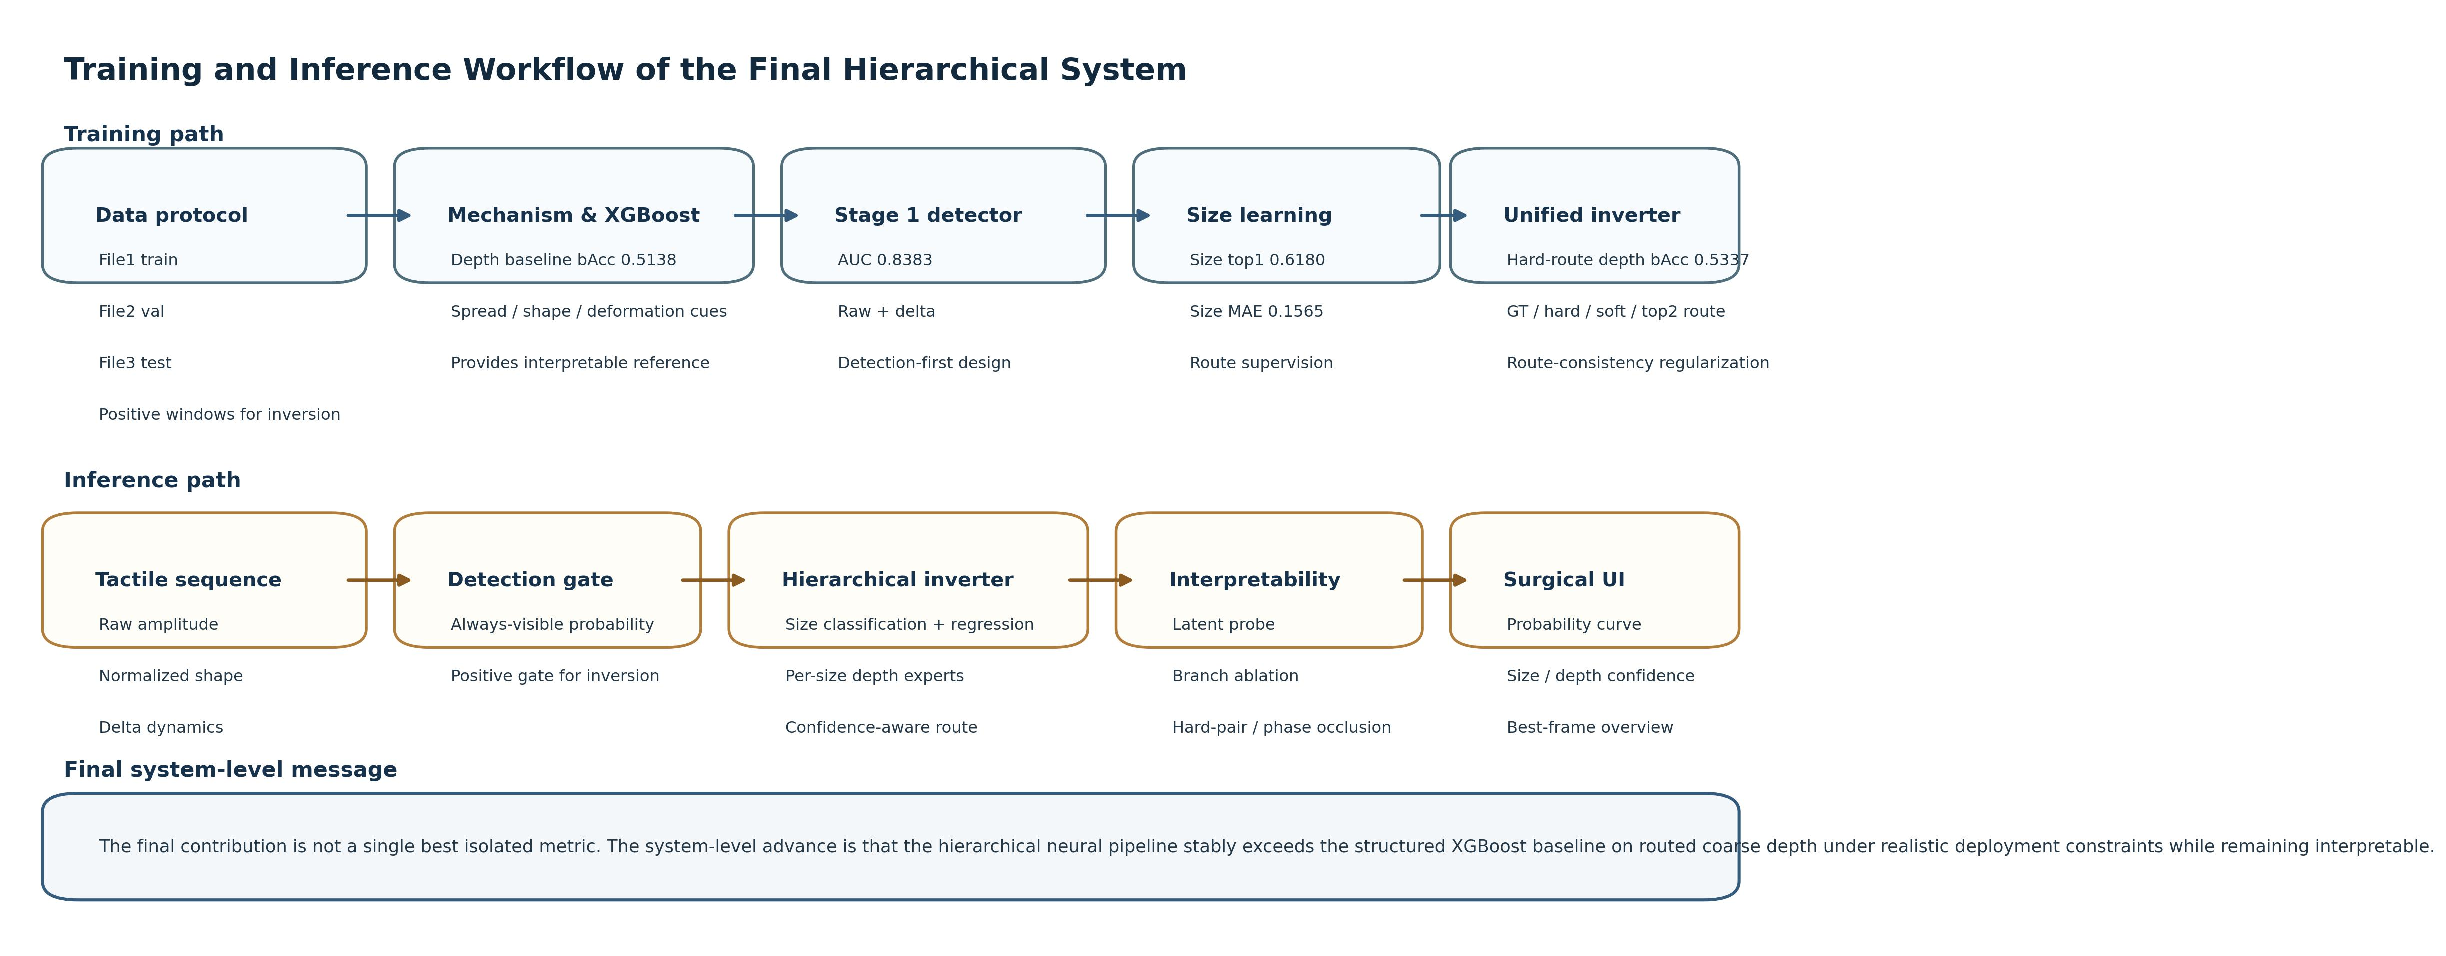
\includegraphics[width=\textwidth]{Fig2_training_inference_pipeline.pdf}
    \caption{Method overview, including the tactile sensing setup, experimental preparation, window-based preprocessing, and the hierarchical inference workflow. The pipeline is organized as Detection $\rightarrow$ Size $\rightarrow$ Depth rather than as parallel outputs.}
    \label{fig:pipeline}
\end{figure*}

\subsection{Raw-Input Hierarchical Neural Pipeline}
\subsubsection{Stage I: Nodule Detection}
The first-stage detector consumed raw spatiotemporal tactile tensors and predicted whether a nodule was present under the current window. The architecture used dual streams for raw and delta inputs, lightweight frame-wise spatial encoding, multiscale temporal convolution, and temporal attention pooling.

\subsubsection{Stage II: Size Inversion}
On true positive windows, we trained a dedicated raw-input size-only router for seven-way size classification and continuous size regression. The purpose of this stage was not to produce the final deployment-optimal size regressor, but to test whether the original tactile tensors already contained strong size information.

\subsubsection{Stage III: Size-Aware Coarse Depth Classification}
Depth was modeled as a three-class coarse discrimination task (\emph{shallow}, \emph{middle}, \emph{deep}) rather than continuous depth regression. Instead of a shared depth head, we used size-routed depth experts. This design directly encoded the physical assumption that depth should be modeled under the size condition rather than as an independent parallel label.

\subsubsection{Design Rationale}
Three complementary tensor views were retained: raw amplitude to preserve absolute intensity and energy, normalized shape to emphasize morphology and spread, and delta sequences to represent local temporal change. The central architectural choice was not deeper stacking, but the explicit reformulation of depth as a size-aware routed task.

\subsection{Interpretability Analysis for the Raw-Input Scientific Model}
To test whether the raw-input depth model automatically encoded physically meaningful structure, we applied three types of analysis: latent linear probes, hard-pair analysis, and phase occlusion. These analyses were used to answer the scientific question of what the raw-input model learned, not to boost deployment performance.

\subsection{Deployment-Oriented Unified Hierarchical Inverter}
In addition to the scientific raw-input model, we built a deployment-oriented unified hierarchical inverter that fused raw amplitude, normalized shape, delta, and structured physical features. This model jointly optimized size classification, ordinal size prediction, size regression, and routed depth under multiple route conditions, including ground-truth route, hard predicted route, soft predicted route, and top-2 route. Its role was system enhancement rather than proof of raw-input automatic learning.

\section{Results}

\subsection{Mechanism Analysis and XGBoost First Established an Information Hierarchy}
Mechanism-guided feature analysis indicated a clear hierarchy in the tactile data: detection-related differences were strongest, size acted as a dominant main effect, and depth appeared as a weaker signal that was easily masked by size. XGBoost converted this into learnability evidence by achieving detection AUC 0.8199, size top-1/top-2 of 0.6701/0.8023 with MAE 0.1472 cm, and coarse depth balanced accuracy 0.5138.

\begin{figure*}[t]
    \centering
    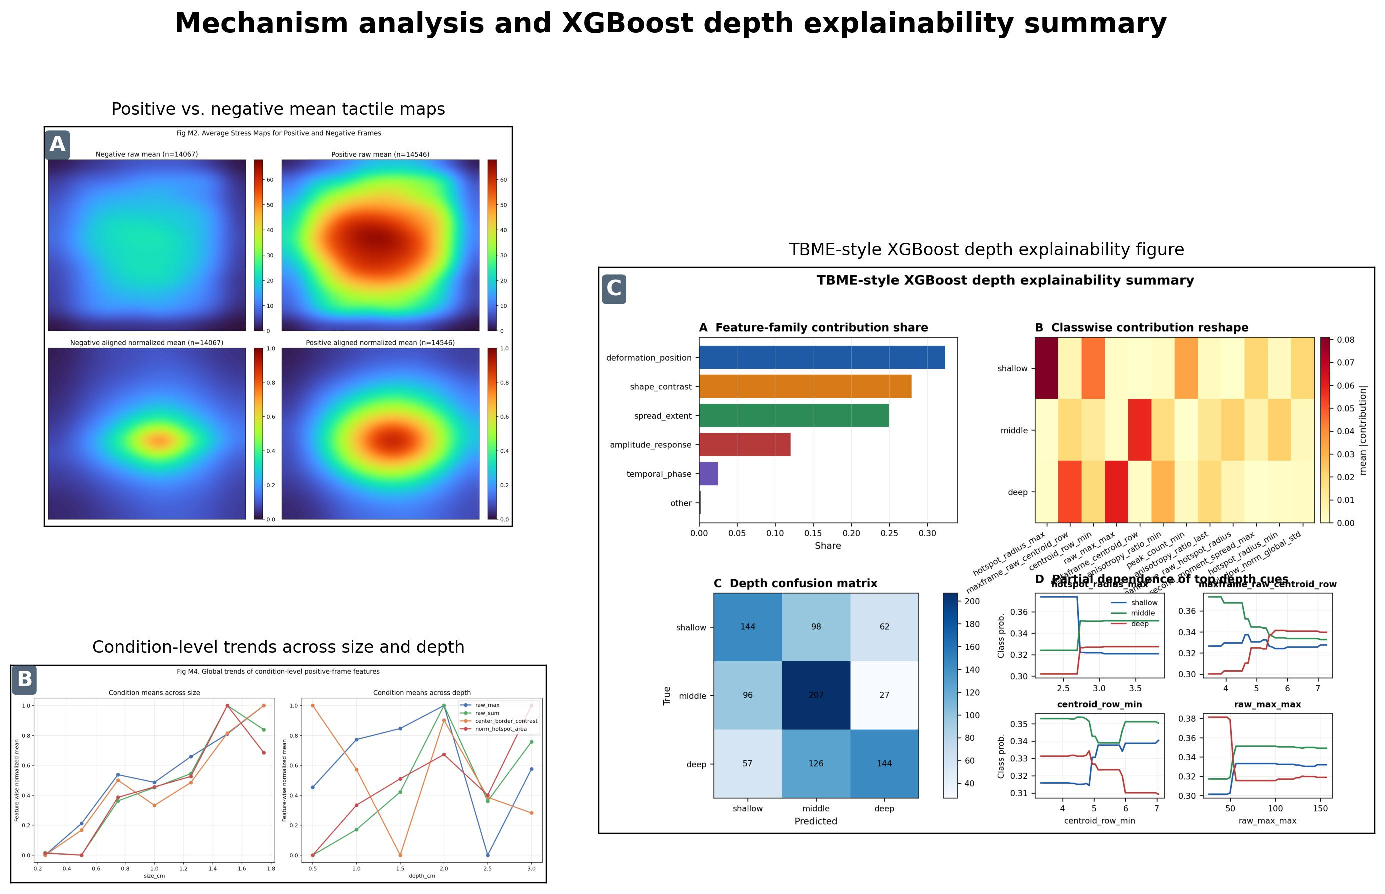
\includegraphics[width=\textwidth]{Fig9_mechanism_xgboost_summary.pdf}
    \caption{Mechanism-guided feature analysis and XGBoost explainability jointly show that the tactile data contain learnable detection, size, and coarse depth information. Depth discrimination is driven more by spread, shape, deformation-position, and phase-related features than by peak amplitude alone.}
    \label{fig:xgb_mechanism}
\end{figure*}

\subsection{Raw-Input Detection Outperformed the Structured Baseline}
On the independent test set, the raw+delta detector reached AUC 0.8383, AP 0.5357, and F1 0.6216, exceeding the XGBoost detection baseline (0.8199, 0.5063, and 0.6185, respectively). This result established that raw spatiotemporal tactile tensors alone were sufficient for reliable intraoperative detection.

\begin{table}[t]
\caption{Detection results on the independent test set.}
\label{tab:detection}
\centering
\begin{tabular}{lccc}
\toprule
Model & AUC & AP & F1 \\
\midrule
XGBoost structured baseline & 0.8199 & 0.5063 & 0.6185 \\
Stage I raw+delta detector & \textbf{0.8383} & \textbf{0.5357} & \textbf{0.6216} \\
\bottomrule
\end{tabular}
\end{table}


\begin{figure}[t]
    \centering
    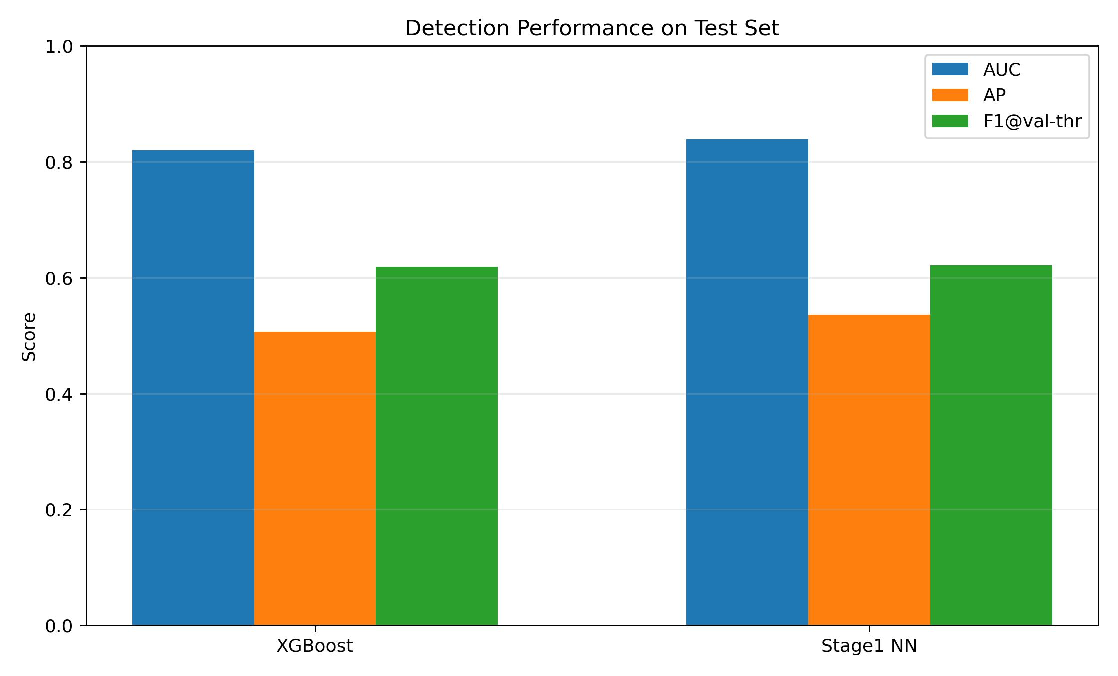
\includegraphics[width=\columnwidth]{Fig4_detection_comparison.pdf}
    \caption{Detection comparison between the structured XGBoost baseline and the raw-input detector. The raw-input detector performs better on the primary task of nodule detection.}
    \label{fig:detection_compare}
\end{figure}

\subsection{Optimized Raw Size Learning Surpassed the Structured Baseline}
After restructuring the pure raw-input size head into a classification--ordinal--expectation--residual form, the raw size-only router reached top-1 0.7177, top-2 0.8195, and MAE 0.1242 cm. This exceeded the XGBoost size baseline (0.6701/0.8023/0.1472), showing that the original tactile tensors themselves were sufficient not only for strong size classification but also for competitive continuous size estimation.

\begin{table}[t]
\caption{Size inversion results on true positive windows.}
\label{tab:size}
\centering
\begin{tabular}{lccc}
\toprule
Model & Top-1 & Top-2 & MAE (cm) \\
\midrule
XGBoost structured baseline & 0.6701 & 0.8023 & 0.1472 \\
Raw size-only router & 0.6600 & 0.8405 & 0.2907 \\
Unified hierarchical inverter & 0.6180 & 0.7859 & 0.1565 \\
\bottomrule
\end{tabular}
\end{table}


\begin{figure}[t]
    \centering
    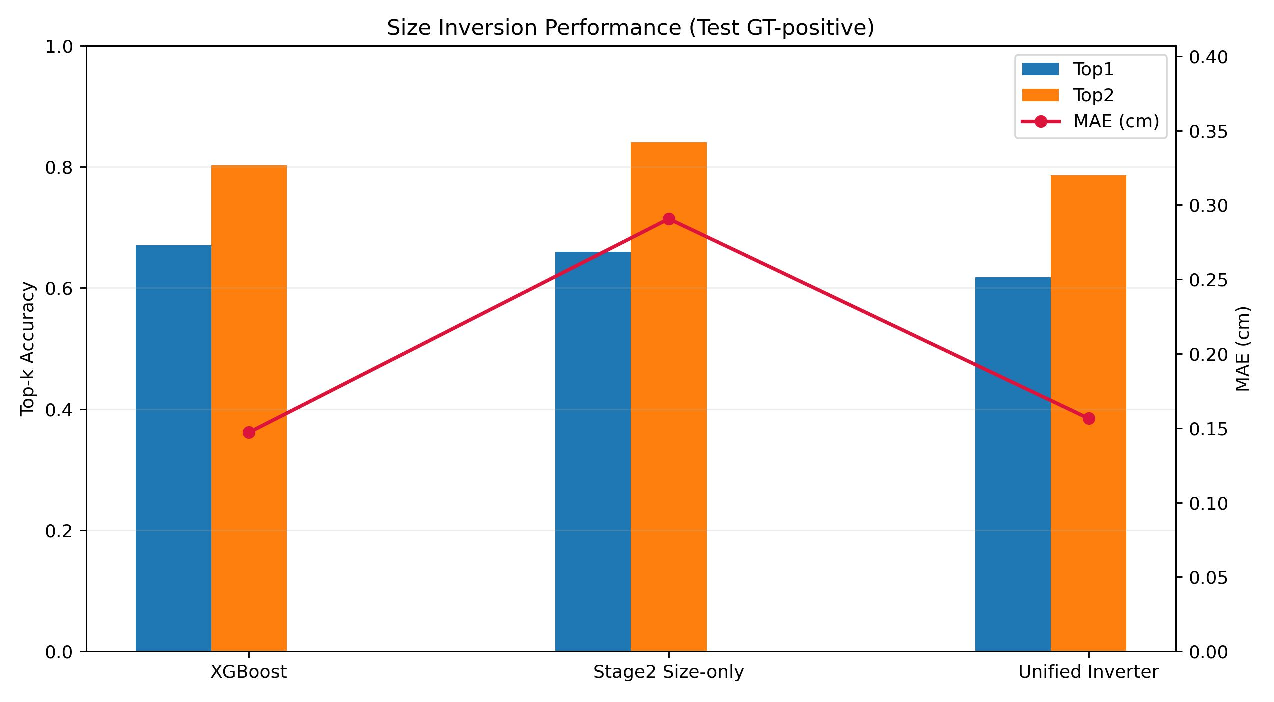
\includegraphics[width=\columnwidth]{Fig5_size_inversion_comparison.pdf}
    \caption{Size inversion comparison. The raw-input size-only model shows strong classification performance, while the structured baseline still retains the best standalone regression MAE.}
    \label{fig:size_compare}
\end{figure}

\subsection{Depth Became Learnable Only Under a Size-Aware Architecture}
When depth was modeled with an ordinary shared head, performance collapsed to near-majority level (balanced accuracy around 0.33). In contrast, a size-routed raw-input depth model improved the ground-truth-route balanced accuracy to 0.5238, slightly above the XGBoost depth baseline of 0.5138. After further introducing route-aware training with a frozen pure raw size router, the ground-truth-route balanced accuracy increased to 0.6066. This result showed that the failure of early raw-input depth models was primarily structural rather than informational.

\begin{table}[t]
\caption{Coarse depth results.}
\label{tab:depth}
\centering
\begin{tabular}{p{0.43\columnwidth}p{0.24\columnwidth}c}
\toprule
Model / Path & Evaluation mode & BAcc \\
\midrule
Majority baseline & GT-positive & 0.3333 \\
XGBoost structured baseline & GT-positive & 0.5138 \\
Raw size-routed depth model & GT route & 0.5238 \\
Raw size-routed depth model & Predicted route & 0.4822 \\
Unified hierarchical inverter & GT route & 0.5407 \\
Unified hierarchical inverter & Predicted hard route & 0.5337 \\
\bottomrule
\end{tabular}
\end{table}


\begin{figure}[t]
    \centering
    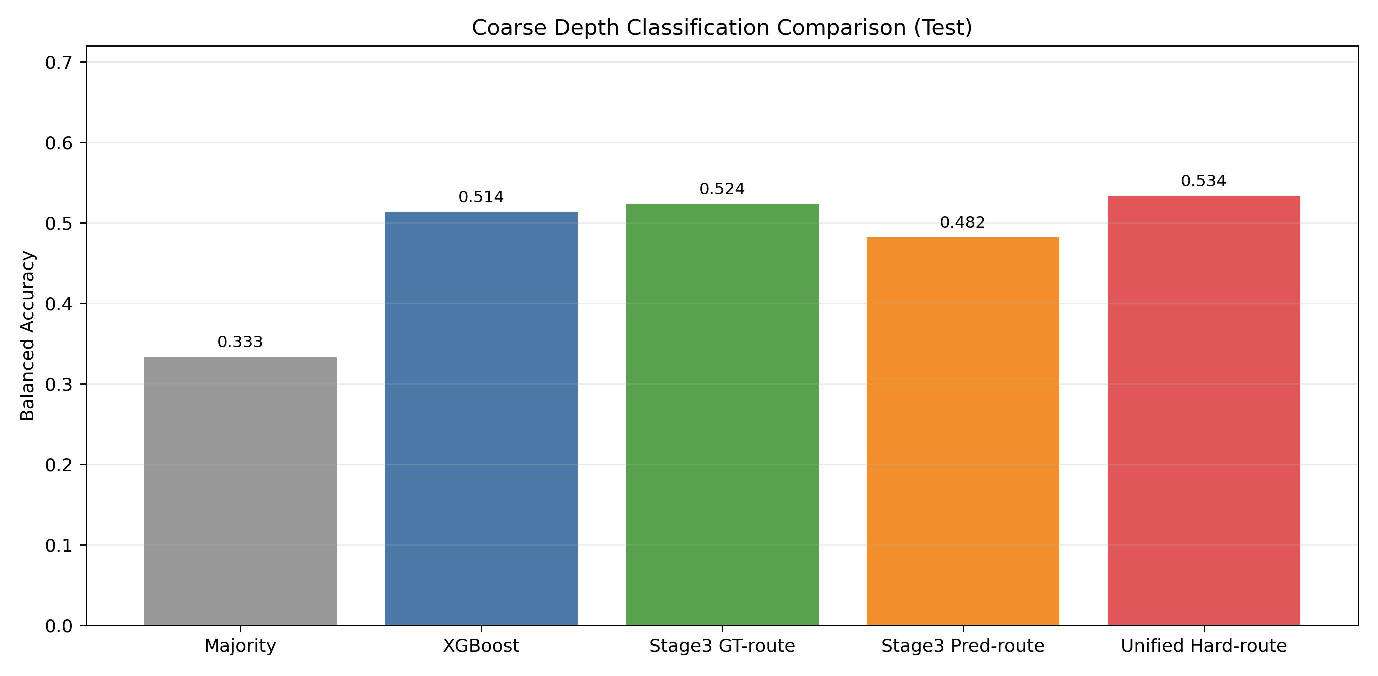
\includegraphics[width=\columnwidth]{Fig6_depth_coarse_comparison.pdf}
    \caption{Coarse depth comparison across majority baseline, XGBoost, and raw-input neural variants. Depth is not learned reliably by a generic shared head, but becomes learnable under a size-aware routed structure.}
    \label{fig:depth_compare}
\end{figure}

\subsection{Interpretability Supported Automatic Encoding of Physical Structure}
Latent probes showed that the raw-input depth model encoded part of the physically meaningful structure beyond size identity alone. Hard-pair analysis indicated that the model was not merely relying on peak amplitude, while phase occlusion revealed that the current time strategy still emphasized the peak neighborhood more than earlier loading or release phases. Together, these analyses supported the claim that raw-input learning had captured part---but not all---of the relevant physical structure.

\begin{figure}[t]
    \centering
    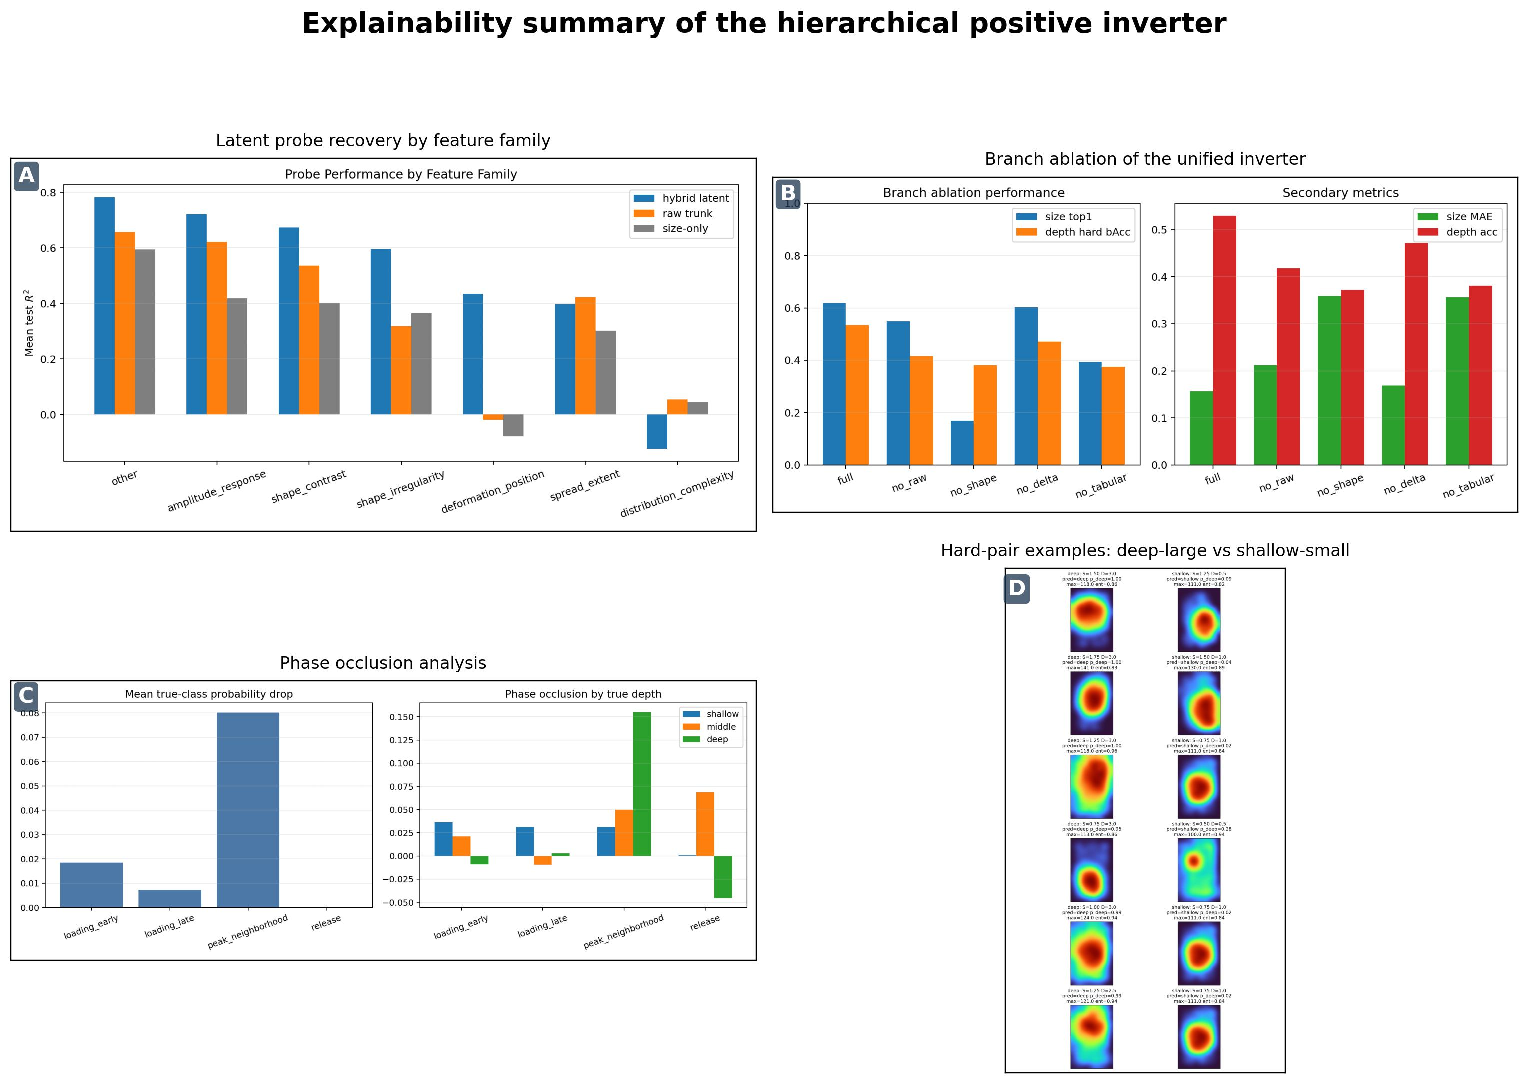
\includegraphics[width=\columnwidth]{Fig10_hierarchical_explainability_summary.pdf}
    \caption{Interpretability summary for the neural pipeline. The model encodes structure related to size and depth, although its temporal strategy remains partially biased toward the peak neighborhood.}
    \label{fig:explainability}
\end{figure}

\subsection{The Main Deployment Bottleneck Was Routing Error Rather Than the Depth Trunk}
Although the first raw size-routed depth model performed well under oracle routing, predicted-size routing reduced depth balanced accuracy to 0.4822. After strengthening the pure raw size router and explicitly training the depth model under ground-truth, hard predicted, soft, and top-2 routing conditions, the pure raw predicted-route balanced accuracy improved to 0.5240. This exceeded the XGBoost depth baseline of 0.5138 and showed that routing robustness, rather than depth information scarcity alone, was the dominant deployment bottleneck.

\subsection{The Unified Hierarchical Inverter Further Improved Predicted-Route System Performance}
The deployment-oriented unified hierarchical inverter directly optimized route-aware performance and improved predicted-route hard balanced accuracy to 0.5337. This exceeded the previous raw predicted-route chain (0.4822), the improved pure raw route-aware chain (0.5240), and the XGBoost depth baseline (0.5138), showing that structured deployment enhancement could further improve the robustness of the full system.

\subsection{Real-Time Display and Latency Supported Practical System Organization}
The real-time interface continuously displayed tactile maps and detection probability, while size and depth outputs were released only under high-confidence conditions. Latency results further showed that although the XGBoost model-only prediction was faster on CPU, explicit structured feature extraction increased the end-to-end burden of the detection pipeline. In contrast, the raw-input detector reached 7.1143 ms on CPU and 2.8131 ms on GPU in the end-to-end setting, making it more suitable for a detection-first online route.

\begin{table}[t]
\caption{Latency benchmark under different measurement scopes.}
\label{tab:latency}
\centering
\begin{tabular}{p{0.40\columnwidth}p{0.26\columnwidth}c}
\toprule
Pipeline & Scope & Median (ms) \\
\midrule
\multicolumn{3}{l}{\textit{Detection path}} \\
XGBoost detection & Model-only CPU & \textbf{0.5740} \\
NN detection & Model-only CPU & 6.9379 \\
XGBoost detection & End-to-end CPU & 27.3447 \\
NN detection & End-to-end CPU & \textbf{7.1143} \\
NN detection & End-to-end GPU & \textbf{2.8131} \\
\midrule
\multicolumn{3}{l}{\textit{Full chain}} \\
XGBoost cascade & End-to-end CPU & \textbf{9.4641} \\
NN two-stage & End-to-end CPU & 14.6890 \\
NN two-stage & End-to-end GPU & 14.5371 \\
\bottomrule
\end{tabular}
\end{table}


\begin{figure}[t]
    \centering
    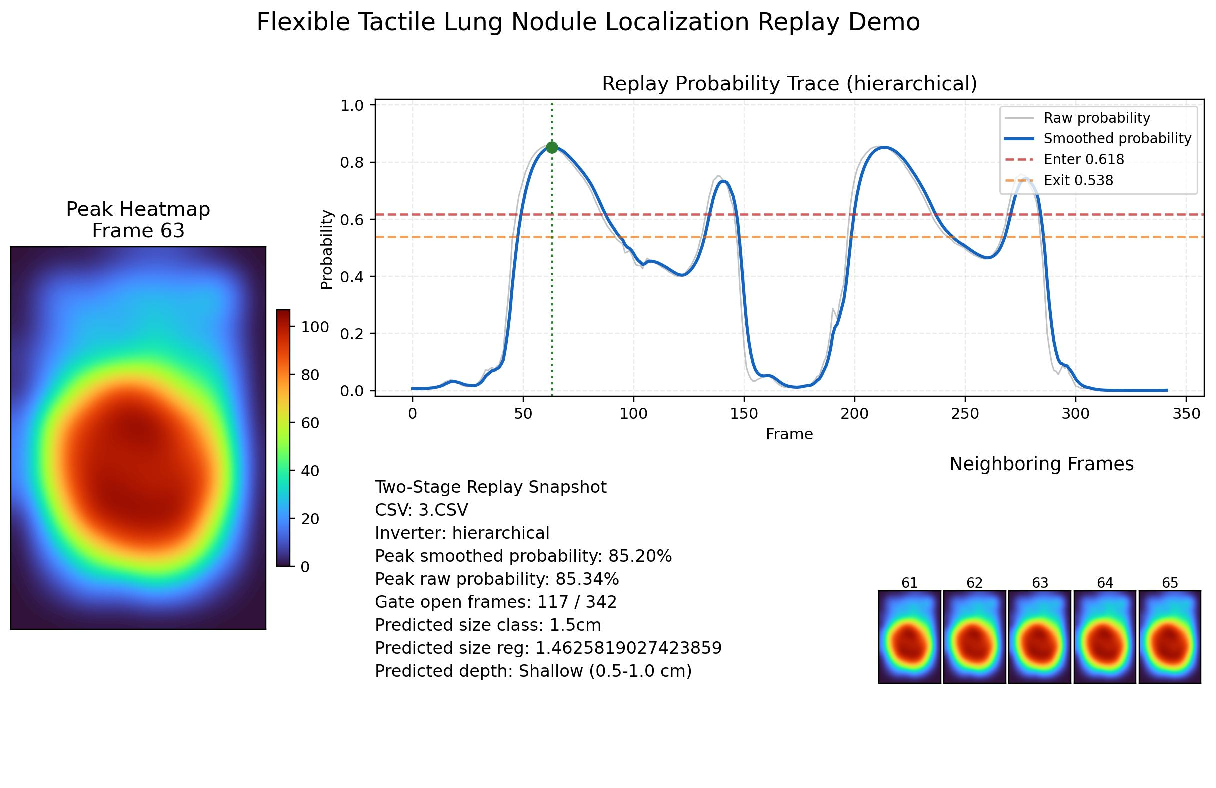
\includegraphics[width=\columnwidth]{Fig12_gui_snapshot.pdf}
    \caption{Real-time interface prototype. Detection remains continuously visible, whereas size and depth outputs are displayed under high-confidence conditions, matching the proposed detection-first system logic.}
    \label{fig:gui}
\end{figure}

\section{Discussion}

The main message of this study is not that neural networks dominate XGBoost on every metric. Rather, the evidence supports a more clinically meaningful interpretation: tactile spatiotemporal data can first support reliable intraoperative nodule detection, then support size inversion, and under explicit hierarchical organization, support coarse depth discrimination. This distinction matters because it aligns the modeling strategy with the actual priority order of intraoperative use.

The strength of the present work lies in the way the problem was organized. We did not force all targets into a flat multitask setting. Instead, we used the signal hierarchy revealed by mechanism analysis: detection as the strongest and most actionable signal, size as a strong secondary signal, and depth as a weaker conditional signal that must be modeled under size awareness. This task reorganization turned out to be more important than simply increasing network complexity.

The study also suggests that XGBoost and neural networks should not be framed as interchangeable competitors. XGBoost first answered whether the tactile data contained learnable information and which physical feature families were most relevant. The raw-input neural pipeline then answered whether the original tensors themselves could support learning without directly feeding those handcrafted physical features into the scientific main model. Finally, the unified hierarchical inverter addressed the engineering question of how to improve predicted-route robustness under realistic deployment conditions.

This role separation is important for interpretation. The raw-input hierarchical neural model should be regarded as the scientific main model because it provides the strongest evidence that original tactile tensors can support detection, size learning, and size-aware coarse depth discrimination, while also enabling interpretability analysis. By contrast, the unified hybrid inverter should be regarded as a deployment enhancement model. Because it explicitly integrates structured physical features, it is well suited for system robustness improvement, but it should not be used as the sole evidence that all physical structure was learned automatically from raw input.

Another practical insight is that the best intermediate metric is not equivalent to the best system-level route. For example, XGBoost still achieved the best standalone size regression MAE, but the unified hierarchical inverter produced the best predicted-route depth performance. This indicates that for intraoperative use, optimizing a single subtask in isolation is less important than improving the robustness of the full decision chain under real routing uncertainty.

Depth remains the most delicate part of the study. The evidence supports the existence of learnable depth information, but only at the level of coarse depth discrimination and only under explicit size-aware organization. The phase-occlusion results also suggest that the current raw-input model still relies more on peak-neighborhood information than on the full loading/release dynamics implied by the mechanism analysis. For this reason, we intentionally avoid framing the present work as a mature continuous depth inversion system.

The study has several limitations. First, the raw-input models did not surpass the structured baseline on every size metric, particularly in standalone regression MAE. Second, depth was limited to a three-class coarse formulation rather than continuous inversion. Third, the experiments were performed on ex vivo porcine lungs rather than clinical intraoperative data. Fourth, the interpretability results should be read as evidence of partial mechanistic consistency, not as a complete recovery of the underlying biomechanics. Future work should strengthen phase-aware modeling, improve route-noise robustness, and test the system under more clinically realistic variability.

\section{Conclusion}

We presented an exploratory intraoperative pulmonary nodule localization framework based on tactile sensing and deep learning, organized around a detection-first logic. The results show that flexible tactile spatiotemporal sensing can support reliable nodule detection, can further support size inversion, and under explicit hierarchical organization, can enable coarse depth discrimination. Mechanism-guided analysis and XGBoost first established that the tactile data contained learnable information; raw-input hierarchical neural models then showed that the original tensors themselves could support learning; interpretability analyses further indicated that the neural representations encoded part of the physically meaningful structure; and a deployment-oriented unified inverter improved predicted-route robustness for system integration. Taken together, these results support the feasibility of a tactile sensing route for intraoperative pulmonary nodule localization while defining a clear boundary: this work should be read as a validated engineering and system-organization pathway rather than a finalized clinical system.


\bibliographystyle{IEEEtran}
\bibliography{references}

\end{document}
